\section{Problemstellung}
\label{problemstellung}

Die vorliegende Arbeit beschäftigt sich mit dem maschinellen Lernen mittels neuronaler Netze \bzw{} Convolutional Neural Networks auf Graphrepräsentation von Bildern.
Als eine \emph{Graphrepräsentation eines Bildes} verstehen wir dabei die Abbildung eines Bildes in einen Graphen, welcher das korrespondierende Bild mittels einer Menge von Knoten und Verbindungen von Knotenpaaren beschreibt, sodass signifikante Merkmale des Bildes erhalten bleiben.
Knoten des Graphen müssen dabei nicht für alle Pixel eines Bildes existieren, sondern können auch ganze Bildbereiche abdecken.
Das bietet sich insbesondere dann an, wenn das vorliegende Bild zu großen Teilen aus Hintergrundbereichen besteht, welche für das Training eines neuronalen Netzes lediglich mehr Aufwand, aber keinen Mehrwert bedeuten.
Damit kann sich folglich für Bilder eine nicht unerhebliche Datenreduktion ergeben, die unter anderem das Potential besitzt, schnellere Ausführungszeiten eines neuronalen Netzes zu garantieren.
Dabei wird das Bild folglich von einer regulären Gitterstruktur in eine irreguläre Graphstruktur übertragen (\vgl{} Abbildung~\ref{fig:problemstellung}).
\begin{figure}[t]
\centering
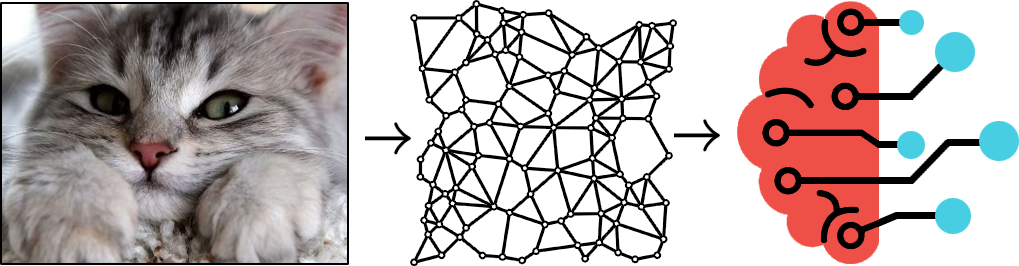
\includegraphics[width=0.9\textwidth]{bilder/problemstellung.png}
\caption[Problemstellung]{Bilder werden in dieser Arbeit für ihre Eingabe in ein neuronales Netz zuvor in eine korrespondierende Graphrepräsentationen konvertiert\protect\footnotemark.}
\label{fig:problemstellung}
\end{figure}
\footnotetext{\url{https://www.shutterstock.com/g/ArtRoseStudio}}

Das Lernen auf solch einer Graphstruktur ist eine sowohl theoretisch als auch implementierungtechnisch herausfordernde Aufgabe, denn schließlich kann der lediglich auf regulären Strukturen definierte klassische Faltungsoperator der Convolutional Neural Networks nicht genutzt werden.
Vorangegangene Arbeiten zeigen, dass eine Generalisierung des Faltungsoperators auf irregulären Datendomänen zwar möglich ist~\cite{patchy, Defferrard, gcn}, sich diese aber letztendlich aufgrund ihrer zu strengen Generalisierung auf willkürliche Graphen ohne Positionsberücksichtigung der Knoten und ihrer in Folge dessen innewohnenden Rotationsinvarianz für die beschriebende Problemstellung als unzureichend herausstellt.
In dieser Arbeit werden daher für die Ansätze des räumlichen sowie des spektralen Lernens auf Graphen weiterführende Methodiken entwickelt, die es ermöglichen, eine Faltung auf Graphen zu realisieren, sodass deren Knotenpositionen und Kantenausrichtungen (wie oben, unten, links oder rechts) analog zu einer Faltung auf Bildern berücksichtigt werden.
Wir zeigen, dass wir mit Hilfe der entwickelten Methodiken im Kontext von Graphen, deren Kanten eine Orientierung zu Grunde liegt, die bisherigen Faltungsoperatoren auf Graphen signifikant verbessern können.
Die vorgestellten Ansätze sind dabei für Graphen, die aus einem Gitter gewonnen wurden, äquivalent zu der klassischen Faltung auf Bildern und besitzen dabei weiterhin den Vorteil, auch auf irreguläre Datendomänen im euklidischen Raum angewendet werden zu können.
Obwohl das Lernen auf den Graphrepräsentationen der Bilder \bzgl{} ihrer Genauigkeit und Laufzeit (noch) nicht ganz mit den klassischen Verfahren auf den Rohdaten der Bilder konkurrieren kann, so zeigen sich die in dieser Arbeit vorgestellten Ansätze dennoch aufgrund ihrer Datenreduktion und Ausweitung der Anwendungsgebiete als lohnenswert für zukünftige Arbeiten.
